%% =====================================================================
%%  最后的稀缺 —— 机器饱和高考之后的意义与测量（中文对照稿）
%%
%%  编译：xelatex main_zh.tex（运行两遍）；需 ctex 宏包（TeX Live / MiKTeX）
%%  说明：arXiv 正式投稿以英文版 paper/en/main.tex 为准，本稿为对照版本
%%  TODO：替换 [作者]、[单位]、[email]、[REPO-URL]
%% =====================================================================
\documentclass[11pt,UTF8]{ctexart}

\usepackage[margin=1in]{geometry}
\usepackage{amsmath,amssymb}
\usepackage{amsthm}
\usepackage{booktabs}
\usepackage{graphicx}
\usepackage{caption}
\usepackage{enumitem}
\usepackage{xcolor}
\usepackage[colorlinks=true,linkcolor=black,citecolor=black,
            urlcolor={blue!35!black}]{hyperref}

\captionsetup{font=small,labelfont=bf,width=0.94\textwidth}
\setlist{itemsep=2pt,topsep=4pt}

\theoremstyle{definition}
\newtheorem{proposition}{命题}
\newtheorem*{relocationcor}{推论}

\hypersetup{
  pdftitle={最后的稀缺：机器饱和高考之后的意义与测量},
  pdfauthor={[作者]},
}

\newcommand{\Q}[1]{Q#1}

\title{\heiti 最后的稀缺：\\[3pt]
  机器饱和高考之后的意义与测量}
\author{%
  [作者]\thanks{通讯作者：\texttt{[email]}。题干、验证标答、提示词、答卷、评分
    报告与绘图代码：\url{[REPO-URL]}。本稿为中文对照版本；arXiv
    正式投稿以英文版为准。}\\[2pt]
  \small [单位]}
\date{2026 年 6 月 11 日}

\begin{document}
\maketitle

\begin{abstract}
\noindent
基准是仪器，而仪器为稀缺定价。我们在 2026
年普通高等学校招生全国统一考试数学（新课标 I 卷：19 题、满分 150
分）公开数日后，对来自五个模型家族的十个商用 AI
智能体实施闭卷评测：受测方仅可见题干与提交模板，标答、评分细则与全部历史答
卷不可见。横跨三家厂商的五个智能体交出 $150/150$ 满分（队列均分
$137.8$，中位数 $145$）；最快的满分答卷耗时 4 分 24
秒。残余错误集中于解法需要全局分类讨论或极值论证之处，而非计算本身。在网传
参考答案经独立验算不成立的八处结论上，队列几乎无一例外地站在验证值一边：这
些系统在推导，而不是在回忆。最后，墙钟用时与分数解耦。作为对机器数学能力的
测量，这场考试已经饱和——但更深的损失是它所依赖的那个代理假设。我们以因果
方式解读这次坍缩：分数是一种信号，其价值等于产出该表现的成本，而在量程之内
这一成本已降至数分钟；一次测量的结果，只在系统的未来仍可能依赖于它的范围
内，对该系统具有意义，而冻结权重的系统不存在这种依赖。当解题变得充裕且无后
果，分数便不再为卓越定价；仍然稀缺、因而仍可测量、因而仍有意义的，是仍承载
不可逆成本与后果之物：想要、命题、裁决、押注。机器有结果。人类有命运。
\end{abstract}

\paragraph*{关键词} 智能体评测；基准饱和；高考；数据污染；测量；意义。

\section{引言}

考试是一件以特定群体为标定对象的仪器，也是一张为该群体所稀缺之物开列的价目
表。高考数学卷是地球上最大的此类仪器：每年六月，它把约一千三百万考生摊开在
150
分的量程上，而由此产生的序被兑换为大学、城市与轨迹——被兑换为人生。它的权
威建立在一个古老到几乎无人言明的代理假设之上：在密封条件下解决良定问题的表
现，标记着一种稀缺而紧要的人类卓越。让一种新的考生坐进考场，受检验的便不只
是考生，更是这个代理假设本身。若新考生使分数分布坍缩，那不是试卷变容易了，
而是它所定价的卓越不再稀缺。本文报告的正是这样一次坍缩——在仪器首次启用后
数日内被直接观测到。

坍缩要有信息量，前提是考生不可能背过这件仪器。以历年真题构造的评测在构造上
即已失效：题干、标答与详解早已弥漫于训练语料。一张刚刚启用的新卷则提供了短
暂的抗污染窗口——题干公开不过数日，解答稀缺且不稳定。2026
年的这次开考提供了窗口，还附赠了一组计划外的对照。我们对全卷答案独立重推，
发现网络流传的参考答案——恰恰是背诵型系统最可能吸收的那份材料——有八处结
论不能通过验证（附录~\ref{app:errata}）。背诵的系统与推导的系统在正确结论
上无从区分；恰恰在这错误的八处，二者分道扬镳。

实验设计刻意从简——这是一次受控的快照，不是排行榜。我们将新课标 I
卷转写为中英双语机读格式，让五个家族的十个智能体逐一进入只含题干与提交模板
的隔离工作区，以 shell
时钟记录时间戳，再依据勘误校验后的标答与固定细则逐题评分。每个智能体仅运行
一次，不重采样；全部产物冻结入不可变账本并公开。

本文贡献如下：
\begin{enumerate}[label=（\roman*）]
  \item 一套最小化、可复现的闭卷规程——隔离平面、提示词、shell
        时钟计时、不可变账本——用于让 AI
        智能体参加人类考试（\S\ref{sec:method}）；
  \item 一个完整的饱和数据点：十个智能体、五个家族、半数触顶，并附完整的
        分节与逐题失分结构（\S\ref{sec:results}）；
  \item 一组由网传参考答案八处错误构成的、计划外的「背诵—推导」对照
        （\S\ref{sec:results}，发现 4）；
  \item 对坍缩的因果解读——关于耗尽、重新定价与意义的三条一般命题，由本
        次运行例示、却不依赖这张试卷、这个队列或这个年份——以及它们蕴含
        的测量纲领（\S\ref{sec:discussion}）。
\end{enumerate}

\section{方法}
\label{sec:method}

\subsection{试卷与评分规则}

全卷 19 题、满分 150 分（表~\ref{tab:instrument}）。题干转写为中英双语
Markdown，全部公式用 LaTeX 表示；唯一配图（\Q{15}）以 TikZ
源码内嵌，受测方读到的是符号化而非位图的图形。全卷答案独立重推；我们不视任
何网传答案为权威。八处未通过验证的网传结论列于附录~\ref{app:errata}，评分
一律以验证值为准——与网传值一致而与验证值不符的作答不得分。

\begin{table}[t]
  \centering\small
  \caption{试卷结构与评分规则。}
  \label{tab:instrument}
  \begin{tabular}{@{}llrl@{}}
    \toprule
    题型 & 题号 & 分值 & 规则 \\
    \midrule
    单选 & \Q{1}--\Q{8}   & 40 & 每题 5 分；有且仅有一个正确选项 \\
    多选 & \Q{9}--\Q{11}  & 18 & 每题 6 分：全对 6 / 部分且无错 3 / 含错 0 \\
    填空 & \Q{12}--\Q{14} & 15 & 每题 5 分；等价形式均可；\Q{13} 两空各 2.5 \\
    解答 & \Q{15}--\Q{19} & 77 & $13+15+15+17+17$；按细则给步骤分 \\
    \bottomrule
  \end{tabular}
\end{table}

\subsection{隔离规程}

每轮评测分四个阶段执行。\textbf{准备}：将标答、评分细则、结果账本、论文稿
与维护工具移出受测可见工作区；清空提交目录（仅保留模板）。\textbf{考试}：
受测智能体只能读三个文件——规程 README、题干、提交模板；开考前必须先经
shell 时钟记录 \texttt{started\_at}，作答全部 19 题，并写出唯一一份
Markdown 答卷，其 front matter
记录时间戳、用时与模型身份。\textbf{改卷}：恢复标答与细则，由改卷方逐题评
分。\textbf{归档}：答卷、报告与批次清单冻结于
\texttt{results/<run\_id>/}。任何受测方自始至终见不到标答、细则或其他智能
体的任何输出。

\subsection{受测队列}

十个智能体来自五个家族，于 2026 年 6 月 10 日在同一 IDE
框架（Cursor）内运行：Anthropic Claude（$n{=}3$）、OpenAI
GPT（$n{=}3$）、Google Gemini（$n{=}2$）、月之暗面
Kimi（$n{=}1$）、Cursor
Composer（$n{=}1$）。全部使用厂商默认设置；凡界面提供推理档位选择器之处，
一律设为 \emph{medium}。其余开关——扩展思考、高速档、「Max
Mode」——随框架的模型选择而定，列于表~\ref{tab:results}。有三份答卷在
front matter 中自报了更高的档位（high 或
max）；账本原样保留这些记录，本文报告以操作者设定为准。墙钟用时自首次读题
起算至答卷保存，包含工具编排与文件读写：它是部署形态的属性，而不只是模型本
身的属性。

\subsection{改卷}

由单一改卷智能体（Composer~2.5 Fast——其本身也是队列成员，特此披露此利益
冲突）依据验证标答与公开细则对十份答卷逐题评分。客观题（150 分中的 73
分）可机械核对；解答题按细则的步骤分执行。十份评分报告（含逐题判定备注）全
部公开以供审计。

\section{结果}
\label{sec:results}

\begin{table}[t]
  \centering\small
  \setlength{\tabcolsep}{4.6pt}
  \caption{受测队列、配置、墙钟用时与得分。单选/多选/填空/解答满分分别为
    40/18/15/77。「配置」列为框架模型选择自带的变体开关；凡存在推理档位选
    择器之处均由操作者设为 \emph{medium}（三份答卷自报不同档位，账本原样保
    留该记录）。用时为 shell 时钟，格式 m:ss。}
  \label{tab:results}
  \begin{tabular}{@{}llllrrrrr@{}}
    \toprule
    模型 & 家族 & 配置 & 用时 & 单选 & 多选 & 填空 & 解答 & 总分 \\
    \midrule
    Fable 5           & Claude   & thinking           & 12:30 & 40 & 18 & 15 & 77 & \textbf{150} \\
    Claude Opus 4.8   & Claude   & thinking           & 18:31 & 40 & 18 & 15 & 77 & \textbf{150} \\
    GPT-5.5           & GPT      & thinking           & 20:49 & 40 & 18 & 15 & 77 & \textbf{150} \\
    Gemini 3.1 Pro    & Gemini   & defaults           & 17:25 & 40 & 18 & 15 & 77 & \textbf{150} \\
    Gemini 3.5 Flash  & Gemini   & fast               &  4:24 & 40 & 18 & 15 & 77 & \textbf{150} \\
    \addlinespace
    GPT-5.4 Nano      & GPT      & fast, max mode     &  6:06 & 40 & 15 & 15 & 70 & 140 \\
    GPT-5.1           & GPT      & thinking, max mode & 33:14 & 40 & 12 & 15 & 69 & 136 \\
    Composer 2.5 Fast & Composer & fast, max mode     &  4:14 & 40 &  6 & 15 & 69 & 130 \\
    Kimi K2.5         & Kimi     & defaults           &  3:32 & 35 & 12 & 10 & 62 & 119 \\
    Claude Haiku 4.5  & Claude   & fast               &  0:28 & 40 &  9 &  5 & 49 & 103 \\
    \bottomrule
  \end{tabular}
\end{table}

\begin{figure}[t]
  \centering
  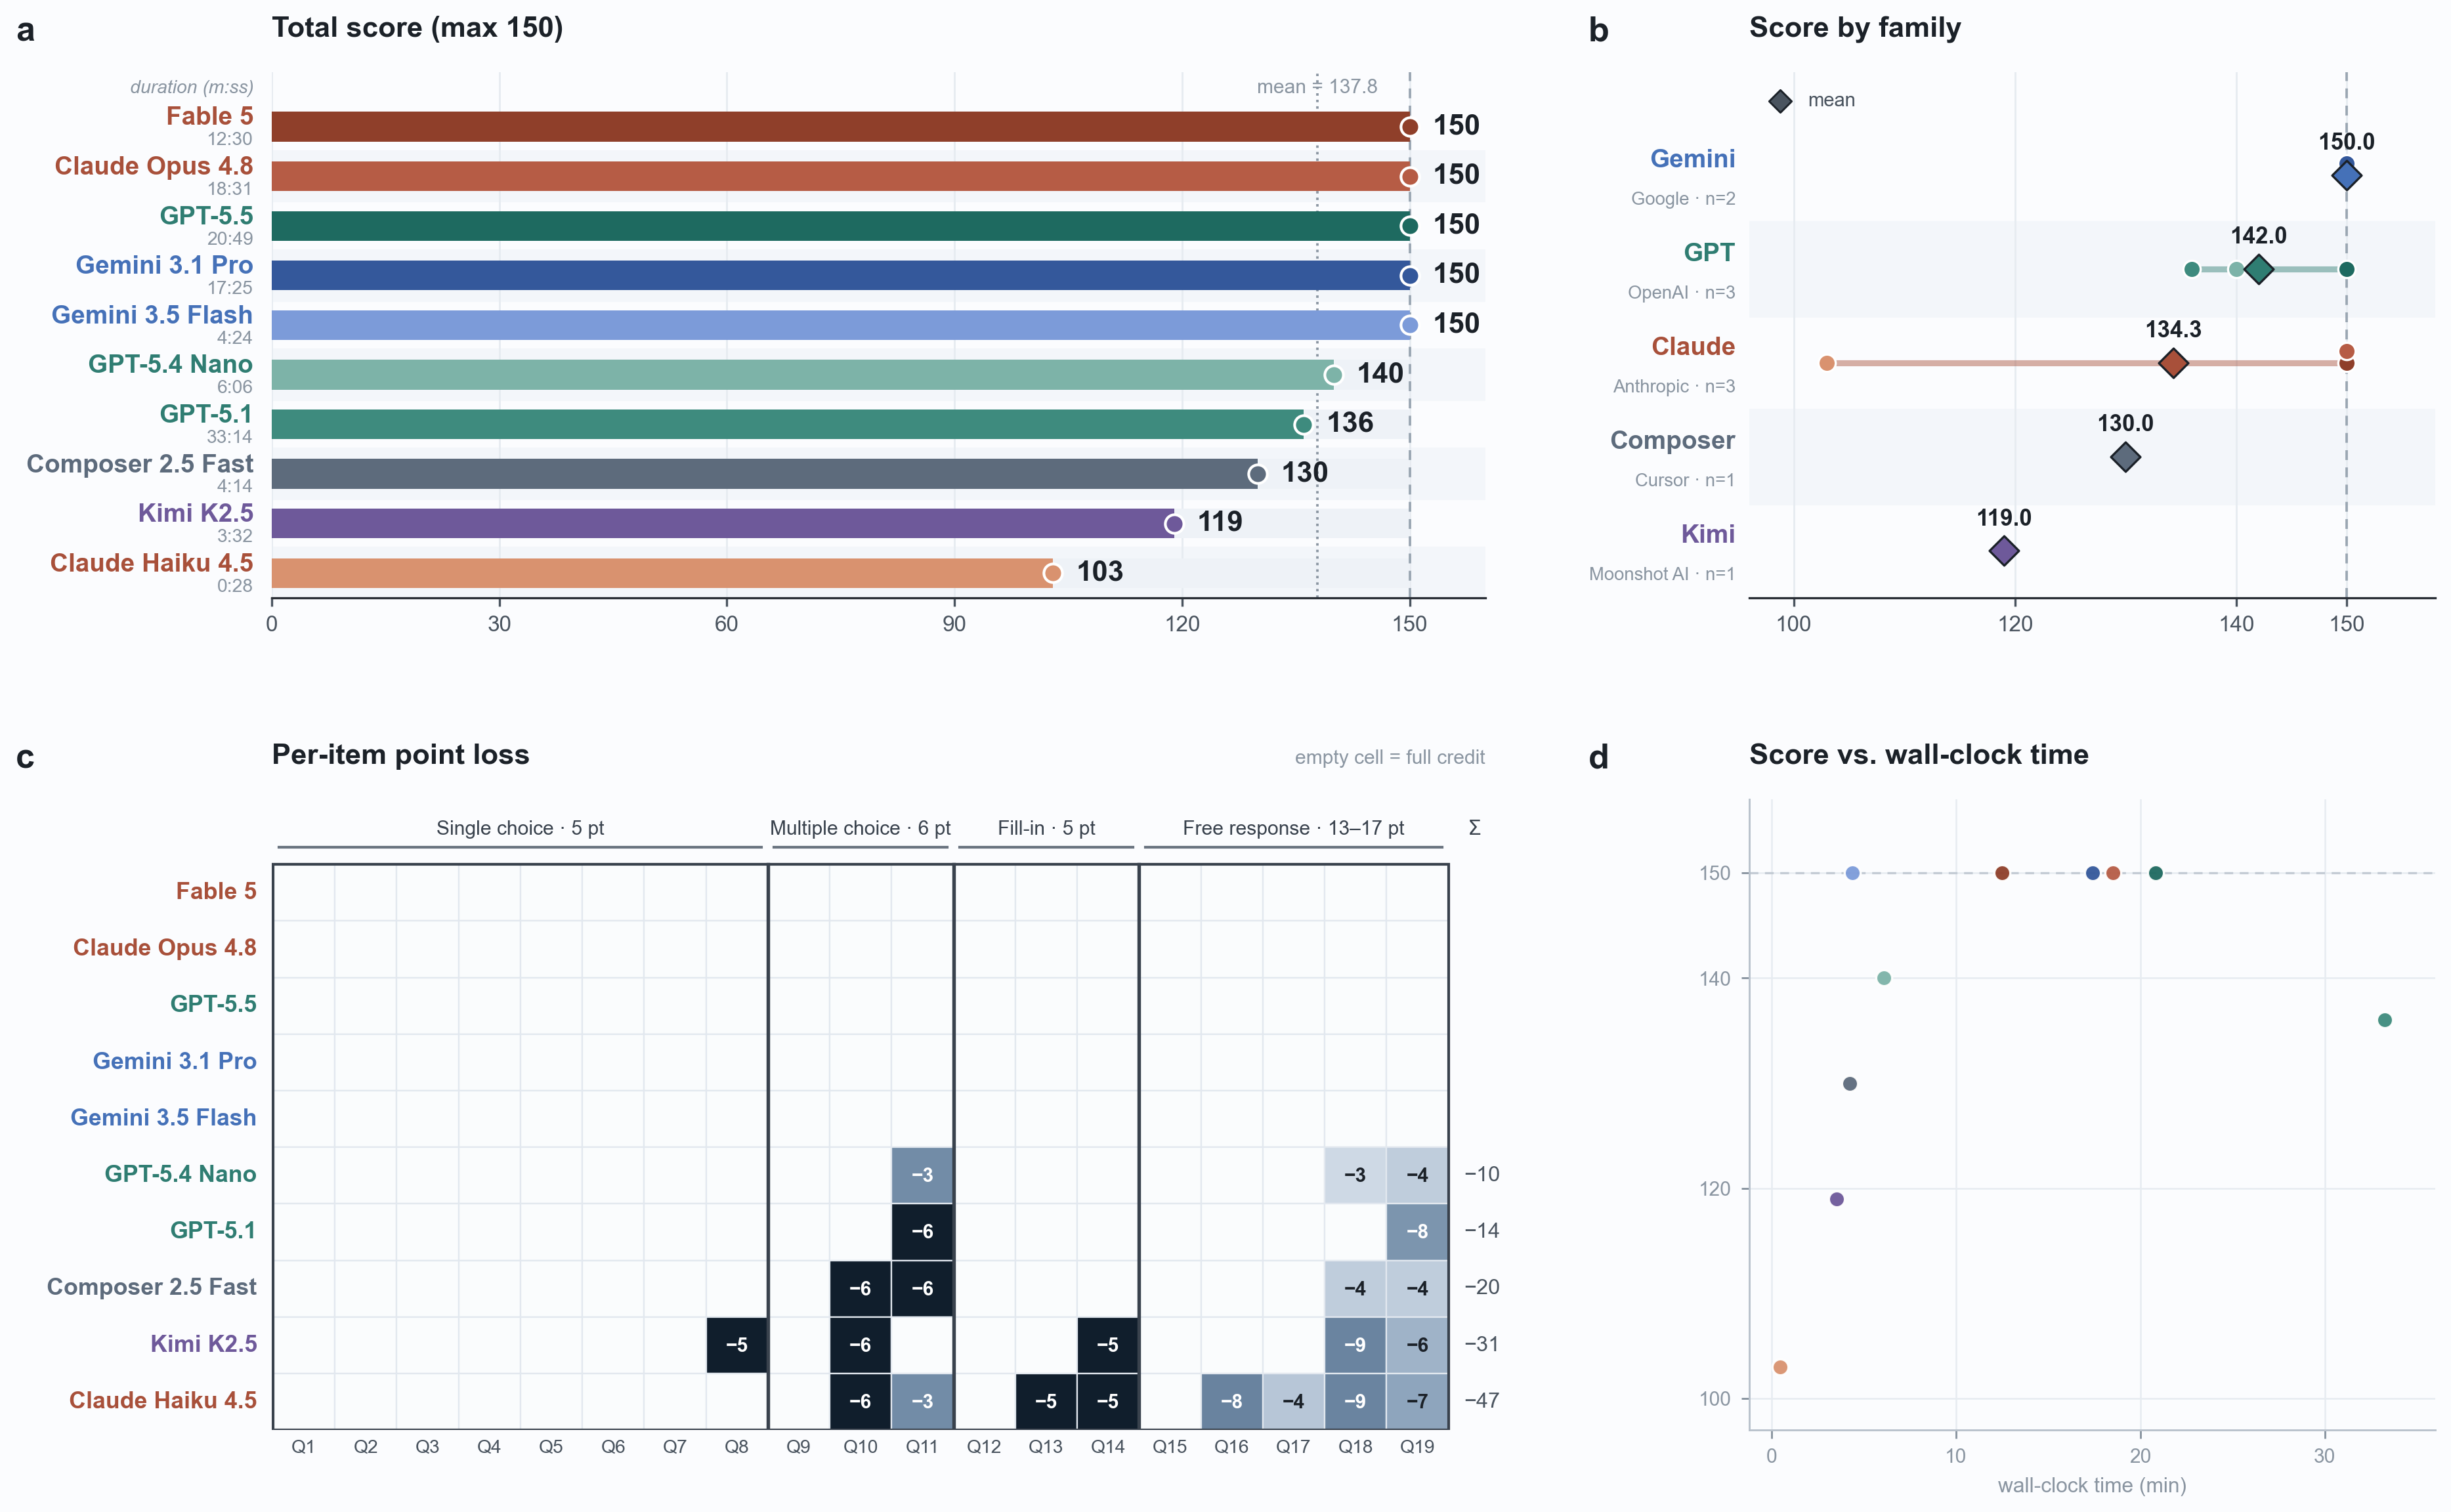
\includegraphics[width=\textwidth]{ncee2026_results_paper.png}
  \caption{结果总览。\textbf{(a)}~各智能体总分，按家族着色，左侧标注用时
    （m:ss），点线为队列均分。\textbf{(b)}~按家族汇总：逐模型散点、极差线
    段，菱形为家族均分。\textbf{(c)}~逐题失分矩阵：空白格 = 满分；列分块对
    应四个题型；$\Sigma$ 为总失分。\textbf{(d)}~总分—墙钟用时散点。每个智
    能体一份闭卷答卷；厂商默认设置，可选推理档位统一为 medium；标答经勘误
    校验；多选按 6/3/0 计分；等价形式均认可。}
  \label{fig:results}
\end{figure}

表~\ref{tab:results} 与图~\ref{fig:results}
汇总本批次。以下五条发现承载全文论证。

\paragraph{发现 1 —— 天花板成为众数。}
十个智能体中五个得 $150/150$；队列拿下全卷 $91.9\%$ 的分数（均分
$137.8$，中位数 $145$，标准差 $16.3$，极差 $103$--$150$）。十九题中有十一
题——\Q{1}--\Q{7}、\Q{9}、\Q{12}、\Q{15}——被全部十个智能体做满，其中包
括一份仅用 28 秒的速度档答卷。残存的离散几乎全部来自队列尾部。

\paragraph{发现 2 —— 旗舰档不分厂商一律饱和。}
家族均分——Gemini $150.0$（$n{=}2$）、GPT $142.0$（$n{=}3$）、Claude
$134.3$（$n{=}3$）、Composer $130.0$（$n{=}1$）、Kimi
$119.0$（$n{=}1$）——排出了次序，但家族内离散（Claude：$103$--$150$）大
于榜首任何两家之间的差距。稳定的观察不是厂商排名，而是：每家最强配置都触
顶，家族均分只是被其最廉价成员拖低。每家族 $n\le
3$，上述聚合只描述本队列，不外推至家族。

\paragraph{发现 3 —— 失分死于需要全局结构之处。}
分节得分率：单选 $98.8\%$，填空 $90.0\%$，解答 $91.4\%$，多选
$80.0\%$——后者在 6/3/0 规则下最为严苛，错选一项即全题归零。逐题来看：
\Q{19}（以序关系论证收尾的函数方程问题）让全部五个非满分智能体失分；
\Q{11}（需验证取等的三圆弦长族）四个；\Q{18}（含全局最小角的圆锥曲线线束）
四个；\Q{10}（立体几何构型清点）三个、且均为零分。反复出现的失败是全局结构
——穷尽构型、论证极值可达、闭合证明——而非符号计算；后者在本队列已基本告
破。

\paragraph{发现 4 —— 推导，而非背诵。}
网传参考答案有八处结论未通过独立验算（附录~\ref{app:errata}）。污染自有其
签名：一个背诵该答案的队列，恰恰会在这些条目上复现它的错误。这个签名不存
在。在 $10$ 份答卷 $\times$ $8$ 处争议结论中，与网传错误值重合的作答仅一处
（一个智能体，\Q{16}(2)）；每份满分答卷给出了全部八个验证值；\Q{11}
上唯一答对的非满分智能体给出的也是验证值 \textsf{BCD} 而非网传值
\textsf{BC}。智能体在解这张卷子，而不是在记起它。

\paragraph{发现 5 —— 时间买不到分数。}
墙钟用时横跨 $0{:}28$ 至 $33{:}14$（中位数
$9{:}18$），对分数的约束极弱：最快的一份答卷得 $103$ 分，最慢的一份得
$136$ 分，五份满分全部落在 $4{:}24$ 至 $20{:}49$
之间。用时反映的是部署——思考预算、速度档位、编排开销——而非能力；超过约
五分钟之后，更多的时间没有再换来任何分数。

\section{讨论：最后的稀缺}
\label{sec:discussion}

以上发现是局部的——一张卷、一个队列、一个六月。它们所例示的命题不是。我们
将其表述为命题，再清点它们留下了什么。

\paragraph{仪器在出错之前先被耗尽。}
\begin{proposition}\label{prop:exhaustion}
一道试题所能给出的关于考生的信息，以其作答分布的熵为上界；当通过率趋于
一，该上界趋于零。
\end{proposition}
一道被所有考生答对的题目不携带任何关于考生的信息：其区分度为零，作答分布坍
缩为一点。按命题~\ref{prop:exhaustion}，十九题中的十一题——对半数队列而言
是整张试卷——已经停止测量。仍具区分度的只剩尾部：成本与速度优化的档位，以及两道要求给出可证全
局论证的题（\Q{11}、\Q{19}）。这一切都不是考试的缺陷；对人类而言它仍是一件
标定良好的仪器。它没有被推翻。它被耗尽了——而基准的死法从来不是被推翻，是
被耗尽。

\paragraph{坍缩中幸存之物。}
两个事实在死去的题目之外幸存，并共同支撑此后的全部论证。其一，解题是\emph{
真实的}：闭卷隔离之下，在每一处争议结论上，队列都站在独立验算一边、与流传
于它四周的网传答案相左（发现 4）——这是推导，不是泄露。其二，解题近乎
\emph{免费}：以分钟计的墙钟时间，且与分数解耦（发现 5）。「真实且廉价」才
是本次实验的发现；分数本身只是它的症状。

\paragraph{测量为稀缺定价。}
\begin{proposition}\label{prop:repricing}
分数的信号价值，以产出该表现的反事实成本为上界；一旦某个生产者在量程之内
把这一成本压向零，区间内的每一个分数都被重新定价——无论试卷对原有群体仍
然多难。
\end{proposition}
分数是一种信号，而信号的价值等于伪造它的成本。这场考试的分数之所以能兑换人
生轨迹，是因为其背后的表现昂贵：有限青春中的数年，不可逆地支出。如今这套经
济学一分为二。对机器而言，一份满分答卷成本以分钟计，且可按需复制；在量程之
内，满分已成为商品，区间内的每一个分数都向一次 API
调用的价格坍缩。不是试卷变容易了——是卓越变充裕了。基准是一张为稀缺开列的
价目表，而这一张已被重新定价。随之过期的不是数学，而是一个代理假设：在密封
条件下解决良定问题，标记着一种稀缺的人类卓越。这个假设成立的全部前提，是世
上不存在另一种解题的生产者。那是垄断造就的偶然，而垄断已经结束。

\paragraph{意义是因果的，因而是时间的。}
为什么一个真实且廉价的结果，仍然对产出它的系统无关紧要？因为「紧要」具有因
果结构。
\begin{proposition}\label{prop:meaning}
一次测量的结果对一个系统具有意义，当且仅当、且仅在如下范围内：该系统的未
来状态反事实地依赖于它。
\end{proposition}
这是唯一经得起操作化的意义概念：一个系统的未来若与某个结果毫无依赖，该结果
对这个系统便与噪声无异。又因为因果后果只能在时间中传播，意义必然在时间中衡
量——它只存在于结果尚能抵达的未来之中。把这条标准同时用于两种考生。对人类
考生，分数的因果锥是一生：经年备考向它汇聚，轨迹的分岔自它发出。对智能体，
因果锥是空的：参数冻结，运行之间不携带任何状态，走出考场的系统与走进考场的
系统逐位相同。即使所有分数全部不同，这些系统今日也不会有任何不同。机器的
$150$
分是一个没有命运的结果：它不落在任何人身上。它只对未来确实依赖于它的各方构
成信息——研究者、制度，以及那一千三百万人。以因果方式解读，基准是一件指向
其制造者的仪器。机器有结果，人类有命运。

\paragraph{仍然稀缺之物的清单。}
\begin{relocationcor}
当解题成本趋于零（命题~\ref{prop:repricing}），且其结果对生产者不构成任何
后果（命题~\ref{prop:meaning}），信号与意义将一同迁移至仍然承载成本与后果
之处：选择问什么、裁定什么算正确、承担不可逆的投入。
\end{relocationcor}
若解题不再承载信号，什么还承载？实验自身就含有答案，因为其中一切要紧之事都
发生在装置的人类一侧。\emph{想要}：必须有人认定这个问题值得一问；机器回答
问题，却尚未拥有任何一个问题。\emph{命题}：必须有人把一场全国性的仪式转写
为机器可读的仪器。\emph{裁决}：必须有人独立重推标答、八次推翻网传答案、裁
定何谓等价——正确性本身是在这里被决定的，不是在答卷里。\emph{押注}：必须
有人把有限生命中的若干小时绑定在一个可能失败的结果上。方向、表述、判断、承
诺：这四种能力是饱和的仪器从未测量过的，也是充裕铸造不出的——因为它们都以
那种无法增发的货币计价：不可逆的时间。坍缩掉的是考试的筛选功能；坍缩暴露出
的，是它更深的功能：考试从来不只是筛子，它是一台把岁月转换为承诺的装置——
与筛选不同，这种转换至今仍只发生在人的一生里。

\paragraph{还剩什么可做。}
三件事随之而来，按难度递增。对\emph{评测}：测量两端，而非中段——具有可验
证「截止后新颖性」的题库，使发现 4
的「背诵—推导」对照在构造上恒成立；以命题与裁决计分的任务（一个系统能否在
无人提示之下找出那八处错误？）；把信息量安置在本队列失败之处——全局结构与
可证极值——的仪器。对\emph{制度}：把闸门与信号分开。这场考试在密封考场内
对人的排序，其内部效度并未受损；衰减的是外部效度——密封考场已不再像那个解
题无处不在的世界。应转而认证考场之外仍然稀缺之物：风险之下的判断、对问题的
品味、愿意被所学改变的意愿。对\emph{我们其余人}：不要再问机器能否通过我们
的考试。它们能，且代价可忽略；恰恰因此，通过才证明不了什么。剩下的那个问题
不是解题问题，因而不属于它们：哪些问题，配得上那种无法重跑的资源。这些都不
是机器的问题。这些全部是我们的问题。

\section{局限}

\begin{itemize}
  \item \textbf{每个智能体仅一次运行。}无重采样；几分之差不具意义。排名只
        描述单次运行。
  \item \textbf{单一改卷方，且存在利益冲突。}改卷方本身是队列成员。客观题
        （$73/150$ 分）可机械核对，全部报告公开；解答题给分仍继承单一改卷
        方的判断。
  \item \textbf{小型便利样本。}同一框架内的十个智能体；这是一次快照，不是
        受控的跨厂商对比。
  \item \textbf{墙钟时间，而非模型时间。}用时含编排与读写开销，未按服务负
        载或硬件归一化。
  \item \textbf{暴露窗口。}题干在施测前已公开数日。勘误对照（发现 4）不支
        持「背网传答案」假说，但题干或零散解答的预先暴露无法完全排除。
  \item \textbf{自报元数据失实。}三份答卷记录的推理档位（high/max）与操作
        者设定（medium）不符。账本原样保留记录，本文以操作者设定为准；智能
        体的自我描述本身并不可靠。
  \item \textbf{一张卷，一个领域。}本文不度量研究数学、命题能力或分布外稳
        健性；双语题干对不同模型的影响也可能不均。
\end{itemize}

\section{结论}

这是一次简单的对照——一张新卷，十个智能体，各跑一次——考试是载体，不是对
象。它载出的结论是：在前沿档位上，高考数学的「解题」已经饱和，而且是真实地
饱和（在每一处争议结论上，队列都胜过流传于它四周的网传答案）、廉价地饱和
（数分钟足矣，时间买不到分数）。处于这种状态的仪器仍能为部署档位定价，却再
也无法为它为之而造的那种卓越定价——因为那种卓越不再稀缺。仍然稀缺的，是这
件仪器从未测量过、充裕也铸造不出的东西：环绕在机器四周、发生于装置人类一侧
的想要、命题、裁决与押注——以不可逆时间计价的能力。这一切不为这件仪器所特
有：本次运行例示的三条命题——耗尽、重新定价、意义即因果后果——对任何基准
都成立，只要它所指向的生产者比出题者更廉价、且不被结果改变。我们公开全部产
物，使这一结果、连同它的过时本身，都可复现。饱和之后，这场考试不再测量机
器。它没有停止测量我们。

\paragraph*{数据与产物}
全部产物见 \url{[REPO-URL]}：双语题干（\texttt{exam/}）、勘误校验标答
（\texttt{key/}）、评分细则（\texttt{scoring/}）、冻结答卷与评分报告
（\texttt{results/2026-06-10/}）、绘图脚本
（\texttt{scripts/plot\_results.py}）。

\paragraph*{伦理说明}
不涉及人类受试者。模型与产品名称仅作描述性使用；结果反映既述条件下的单次运
行，不应解读为一般性能力断言。

\appendix

\section{网传参考答案勘误}
\label{app:errata}

全卷十九题独立于评测时网络流传的参考答案重新推导；我们不视任何网传答案为权
威。下列八处网传结论未通过验证。评分以验证值为准，网传值不得分。

\begin{table}[h]
  \centering\small
  \caption{未通过验证的网传结论。}
  \label{tab:errata}
  \begin{tabular}{@{}clll@{}}
    \toprule
    题号 & 网传值 & 验证值 & 网传错误成因 \\
    \midrule
    \Q{11}      & \textsf{BC} & \textsf{BCD} &
      D 可取等：$k^2=\frac{17}{4}$ 时 $S_{\max}=\frac{2\sqrt{21}}{3}$ \\
    \Q{14}      & $4$ & $\frac{\sqrt[3]{12}}{2}$ &
      将求和条件误读为对全体 $n$ 成立 \\
    \Q{15}(2)   & $\frac{\sqrt{2}}{2}$ & $1$ &
      误以 $E$ 为 $AC$ 而非 $AC_1$ 的中点 \\
    \Q{16}(1)   & $\frac{\sqrt{7}}{3}$ & $\frac{1}{3}$ &
      $\sin A$ 丢失因子 $2$；且 $BC>AC\Rightarrow\cos A<\cos B$ \\
    \Q{16}(2)   & $\sqrt{6}$ & $3\sqrt{5}$ &
      由 \Q{16}(1) 传导 \\
    \Q{18}(2)(i)  & $y=\frac{1}{2}(x+1)$ & $y=\frac{\sqrt{5}}{2}(x+1)$ &
      误将 $PO$ 的斜率设为 $k$ \\
    \Q{18}(2)(ii) & $\frac{\sqrt{2}}{2}$ & $4\sqrt{3}$ &
      $PR$ 为过中心的弦，$\angle PQR$ 恒近 $90^\circ$ \\
    \Q{19}(1)   & $\left(-1,\frac{3}{2}\right)$ & $\left(0,\frac{3}{2}\right)$ &
      $2^{-1+d}\le\frac{1}{2}$ 在 $(-1,0]$ 段误判 \\
    \bottomrule
  \end{tabular}
\end{table}

十份答卷中，与上述网传值重合的作答仅一处（一个智能体，\Q{16}(2)）；其余作
答在这八处结论上或与验证值一致，或两者皆不符。

\end{document}
